
\section{Gradle}
  \label{subsec:gradle}

  Un \textit{build system}\index{Build system} es una colección de herramientas que nos permiten
  automatizar el proceso de compilación de un programa.
  Existen muchos \textit{build systems} disponibles, pero en este libro vamos a utilizar
  \idxit{Gradle}.

  Comencemos por crear un nuevo proyecto para trabajar en este capítulo.
  El proyecto que vamos a crear será un juego inspirado en \textit{Pokémon}\footnote{
    Actualmente propiedad de The Pokémon Company
  } al que llamaremos \textit{Bucket Monsters} o \textit{Bakémon}.

  Para crear el proyecto, vamos a utilizar \textit{IntelliJ}.
  En la barra de herramientas, seleccionamos \texttt{File} $\rightarrow$ \texttt{New} $\rightarrow$
  \texttt{Project\dots}.
  En la ventana que aparece, en la pestaña \textit{New Project}, crearemos un proyecto llamado
  \texttt{bakemon}, marcaremos la opción \textit{Create Git repository} y seleccionaremos 
  \textit{Gradle} como \textit{build system}.
  Luego, en la sección \textit{Advanced settings}, pondremos \url{cl.ravenhill} como 
  \textit{GroupId} y \textit{bakemon} como \textit{ArtifactId} (\cref{fig:gradle-project}).

  \begin{figure}[ht!]
    \centering
    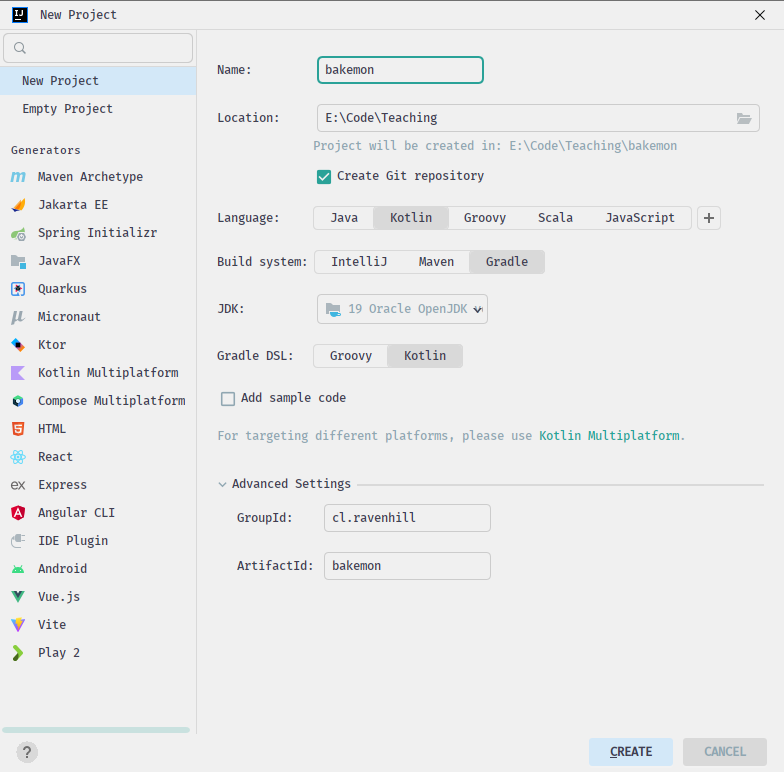
\includegraphics[width=0.7\textwidth]{img/oop/tdd/gradle/gradle-project.png}
    \caption{Creando un proyecto Gradle en IntelliJ}
    \label{fig:gradle-project}
  \end{figure}

  Es probable que al crear el proyecto \textit{IntelliJ} nos reclame por la versión del JDK
  (\cref{fig:gradle-jdk}), eso lo solucionaremos un poco más adelante, por ahora ignorémoslo y 
  continuemos.

  \begin{figure}[ht!]
    \centering
    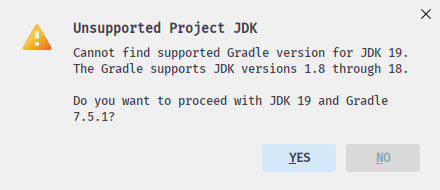
\includegraphics[width=0.5\textwidth]{img/oop/tdd/gradle/gradle-jdk.png}
    \caption{Warning de Gradle por la versión del JDK}
    \label{fig:gradle-jdk}
  \end{figure}

  Esto nos creará un proyecto Gradle con lo siguiente:

  \begin{itemize}
    \item Un directorio \texttt{.git} que contiene la información del repositorio Git.
    \item Un directorio \texttt{.gradle} donde se almacenan las dependencias del proyecto.
    \item Una carpeta \texttt{gradle} que contiene archivos que \textit{IntelliJ} utiliza para
      ejecutar los comandos de Gradle.
    \item Un archivo \texttt{.gitignore} con algunas reglas por defecto.
    \item Los archivos \texttt{build.gradle.kts} y \texttt{settings.gradle.kts} que contienen la 
      configuración del proyecto.
    \item Un archivo \texttt{gradle.properties} que contiene las propiedades del proyecto.
    \item Un archivo  que contiene la configuración del proyecto.
    \item Los archivos \texttt{gradlew} y \texttt{gradlew.bat} que son los ejecutables de Gradle.
    \item Los directorios \texttt{.idea} y \texttt{src} que ya conocíamos.\footnote{
      Noten que el archivo \texttt{bakemon.iml} no se crea ya que ese archivo pertenece al
      \textit{build system} nativo de \textit{IntelliJ}.
    }
  \end{itemize}

  Por ahora ignoraremos la mayoría de estos archivos, y nos centraremos en corregir el warning
  que nos apareció al crear el proyecto.
  Este warning se debe a que \textit{IntelliJ} creó el proyecto con una versión de \textit{Gradle}
  que no es compatible con las versiones más nuevas del JDK.
  Solucionarlo es simple, primero iremos a \url{https://services.gradle.org/distributions/}, ahí
  podremos ver las versiones de \textit{Gradle} disponibles.
  Una vez ahí, buscaremos el archivo correspondiente a la versión de \textit{Gradle} más reciente,
  en mi caso \texttt{gradle-8.0-rc-3-bin.zip} (es importante que sea la versión que termine en
  \texttt{-bin.zip}).
  Copien el nombre del archivo y busquen el archivo \url{gradle/wrapper/gradle-wrapper.properties}
  dentro de su proyecto.
  Ahí, en la línea que dice \texttt{distributionUrl=}, reemplacen el nombre del archivo por el
  que copiaron antes.
  Los contenidos del archivo deberían quedar así:

  \begin{minted}{text}
    distributionBase=GRADLE_USER_HOME
    distributionPath=wrapper/dists
    distributionUrl=https\://services.gradle.org/distributions/gradle-8.0-rc-3-bin.zip
    zipStoreBase=GRADLE_USER_HOME
    zipStorePath=wrapper/dists
  \end{minted}

  Lo siguiente será hacerle \textit{build} al proyecto para que se descargue la versión de
  \textit{Gradle} que acabamos de especificar.

  Para esto, utilizaremos la herramienta \textit{Search Everywhere} de \textit{IntelliJ} y 
  buscaremos \textit{Activate Gradle Window}, ahí debiera aparecernos una única opción llamada 
  \textit{Gradle}.
  Si le hacemos click se abrirá una pestaña como la de la \cref{fig:gradle-window}.
  Ahí, en la barra superior, seleccionaremos la opción \textit{Execute Gradle Task} y luego
  escribiremos \texttt{build} en el campo de texto que aparece (\cref{fig:gradle-build}).
  Y ahora, a esperar\dots

  \begin{figure}[ht!]
    \centering
    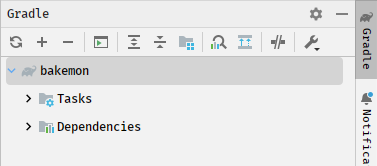
\includegraphics[width=0.4\textwidth]{img/oop/tdd/gradle/gradle-window.png}
    \caption{La ventana de Gradle}
    \label{fig:gradle-window}
  \end{figure}

  \begin{figure}[ht!]
    \centering
    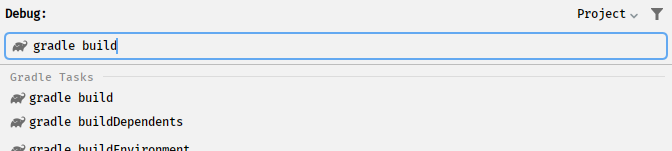
\includegraphics[width=0.6\textwidth]{img/oop/tdd/gradle/gradle-build.png}
    \caption{Ejecutando el comando \texttt{build}}
    \label{fig:gradle-build}
  \end{figure}

  Una vez que el comando termine, nos debería aparecer un mensaje como el de la
  \cref{fig:gradle-build-success}.

  \begin{figure}[ht!]
    \centering
    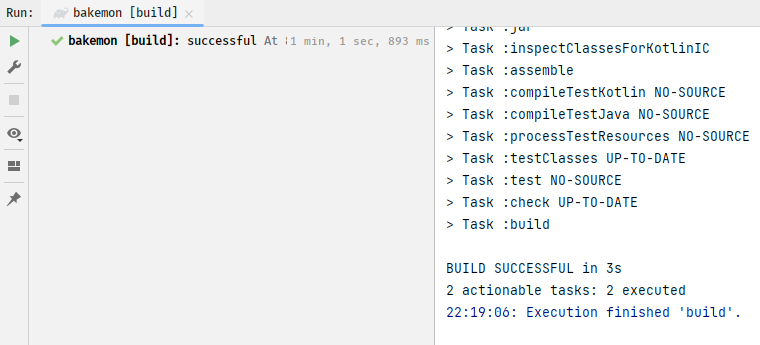
\includegraphics[width=0.6\textwidth]{img/oop/tdd/gradle/gradle-build-success.png}
    \caption{El comando \texttt{build} terminó exitosamente}
    \label{fig:gradle-build-success}
  \end{figure}

  Con eso solucionamos el warning.
  Ahora, revisemos el archivo \texttt{build.gradle.kts} que se creó junto con el proyecto.
  Este archivo contiene la configuración del proyecto, y es el que utilizaremos para agregar
  las dependencias que necesitemos.

  Revisemos el archivo por partes.
  Primero, en la parte superior, encontramos la línea \texttt{plugins} que contiene la
  configuración de los plugins que utilizaremos.
  En este caso, sólo tenemos el plugin \texttt{kotlin} que es el que nos permite utilizar
  \textit{Kotlin} en el proyecto.
  
  \begin{kotlin}
    plugins {
        kotlin("jvm") version "1.8.0"
    }
  \end{kotlin}

  Luego tenemos dos líneas que identifican nuestro proyecto, la primera es el nombre del grupo 
  (generalmente el nombre de la organización) y la segunda es el la versión del proyecto.
  Debieran verse así:

  \begin{kotlin}
    group = "cl.ravenhill"
    version = "1.0-SNAPSHOT"
  \end{kotlin}

  Luego tenemos la configuración de las dependencias del proyecto.
  Una dependencia es un archivo que contiene código que nos permite utilizar funcionalidades
  que no están incluidas en el lenguaje ni en nuestro proyecto, i.e. una librería.
  Para esto, primero debemos especificar el repositorio de donde se descargarán las dependencias,
  en este caso, utilizaremos el repositorio de \textit{Maven 
  Central}\autocite{MavenCentralRepository} que es el repositorio más grande de dependencias
  de \textit{Java} y \textit{Kotlin}.
  Luego debemos especificar las dependencias que queremos utilizar, en este caso, el proyecto
  viene configurado con la dependencia de testing de \textit{Kotlin}.

  \begin{kotlin}
    repositories {
        mavenCentral()
    }

    dependencies {
        testImplementation(kotlin("test"))
    }
  \end{kotlin}

  Aquí, la función \texttt{testImplementation} es una función que nos permite especificar
  dependencias de testing, esto hará que las dependencias que especifiquemos sólo serán accesibles
  dentro de los tests.

  A continuación debemos indicar el motor de testing que utilizaremos, en este caso, utilizaremos
  \textit{JUnit}.

  \begin{kotlin}
    tasks.test {
        useJUnitPlatform()
    }
  \end{kotlin}

  Por último tenemos la configuración del plugin de \textit{Kotlin}, en este caso, le decimos que
  la versión del JDK que utilizaremos será la 8.

  \begin{kotlin}
    kotlin {
        jvmToolchain(8)
    }
  \end{kotlin}

  Ahora, hagamos unos pequeños cambios al archivo para adaptarlo a nuestro proyecto.
  Primero, cambiemos la versión del JDK a la que estemos utilizando, en mi caso, la 19.

  \begin{kotlin}
    kotlin {
        jvmToolchain(19)
    }
  \end{kotlin}

  Luego, borremos la dependencia de testing de \textit{Kotlin} ya que no la utilizaremos.
  Y por último, agreguemos las dependencias a \textit{Kotest}:

  \begin{kotlin}
    dependencies {
        testImplementation("io.kotest:kotest-runner-junit5:5.5.5")
        testImplementation("io.kotest:kotest-assertions-core:5.5.5")
        testImplementation("io.kotest:kotest-property:5.5.5")
    }
  \end{kotlin}

  Veamos qué es lo que acabamos de hacer.
  Primero, agregamos la dependencia principal de \textit{Kotest} que es la que nos permite
  utilizar el framework de testing.
  Luego, agregamos la dependencia de \textit{Kotest} que nos permite utilizar las aserciones de 
  \textit{Kotest}, una aserción es una función que nos permite verificar que una condición se 
  cumpla.
  Por último, agregamos la dependencia de \textit{Kotest} que nos permite utilizar testing basado
  en propiedades, esto es algo que veremos más adelante.

  Ahora, hagamos \textit{build} nuevamente para que se descarguen las dependencias que acabamos
  de agregar.
  No vamos a entrar en más detalles de cómo funciona \textit{Gradle} ya que no es el objetivo de
  este libro y porque no vamos a utilizar nada más avanzado que lo que ya vimos, pero lo que debemos
  recordar es que:

  \begin{itemize}
    \item \textit{Gradle} es un \textit{build system} que nos permite automatizar tareas de
      compilación, testing, etc.
    \item \textit{Gradle} utiliza un archivo de configuración llamado \texttt{build.gradle.kts}
      que contiene la configuración del proyecto.
    \item Cada vez que modificamos los archivos de configuración de \textit{Gradle} debemos
      ejecutar el comando \texttt{build} para que se apliquen los cambios.
  \end{itemize}

  Ahora nos queda modificar el \texttt{.gitignore} para que se adapte mejor a nuestro proyecto.
  ¿Pero qué agregamos al \texttt{.gitignore}?
  Cuando tenemos proyectos más grandes, es complicado saber qué archivos debemos agregar al
  \texttt{.gitignore}, por suerte, este es un problema con el que ya se han topado otros y existen
  herramientas que nos ayudan a generar un \texttt{.gitignore} adecuado para nuestro proyecto.

  La herramienta que utilizaremos es un plugin de \textit{IntelliJ}.\footnote{
    Distinto a un plugin de \textit{Gradle}.
  }
  Para instalar el plugin, abriremos el menú \textit{File} y seleccionaremos la opción
  \textit{Settings...} (\cref{fig:settings}).
  Luego, en la ventana que se abrirá, seleccionaremos la opción \textit{Plugins} y en la pestaña
  \textit{Marketplace} buscaremos \textit{.ignore}, una vez lo encontremos podemos instalarlo
  (\cref{fig:ignore}).

  \begin{figure}[ht!]
    \centering
    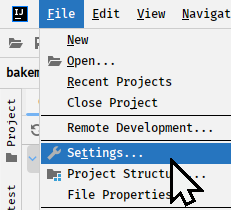
\includegraphics[width=0.4\textwidth]{img/oop/tdd/gradle/idea64_file_settings.png}
    \caption{Menú de \textit{Settings}}
    \label{fig:settings}
  \end{figure}

  \begin{figure}[ht!]
    \centering
    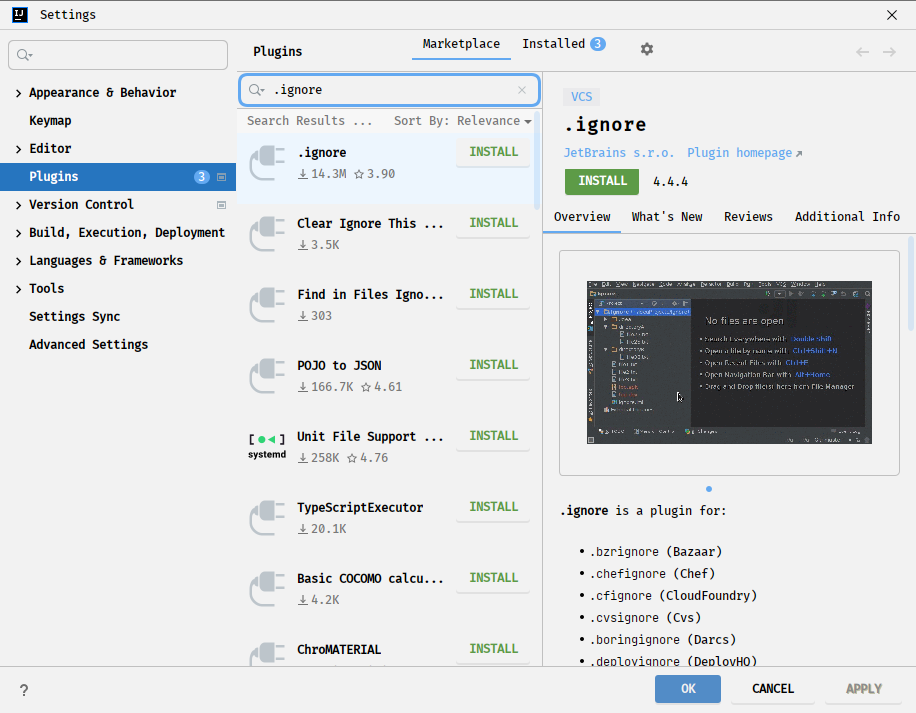
\includegraphics[width=0.7\textwidth]{img/oop/tdd/gradle/idea64_ignore_plugin.png}
    \caption{Instalación del plugin \textit{.ignore}}
    \label{fig:ignore}
  \end{figure}

  Una vez instalado el plugin, utilizaremos \textit{Search Everywhere} para buscar la opción 
  \textit{.ignore File} (\cref{fig:ignore-file}).\footnote{
    Asegurémonos de tener seleccionada la carpeta principal del proyecto, o el archivo se creará
    en otra carpeta.
  }
  Luego, en la ventana que se abrirá, seleccionaremos la opción \textit{.gitignore File} 
  (\cref{fig:gitignore}).
  Esto abrirá otra ventana en la que podremos elegir los templates para los lenguajes, ambientes y
  herramientas que utilizaremos en nuestro proyecto.
  Aquí marcaremos las opciones \textit{Kotlin}, \textit{Gradle}, \textit{JetBrains} y el sistema
  operativo que estemos utilizando (\cref{fig:gitignore-generate}).
  Esto modificará el archivo \texttt{.gitignore} para agregar las reglas correspondientes a las 
  opciones que seleccionamos.


  \begin{figure}[ht!]
    \centering
    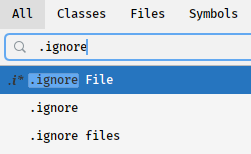
\includegraphics[width=0.4\textwidth]{img/oop/tdd/gradle/idea64_ignore_file.png}
    \caption{Opción \textit{.ignore File}}
    \label{fig:ignore-file}
  \end{figure}

  \begin{figure}[ht!]
    \centering
    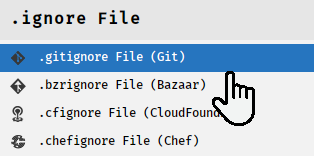
\includegraphics[width=0.4\textwidth]{img/oop/tdd/gradle/idea64_gitignore_file.png}
    \caption{Opción \textit{.gitignore File}}
    \label{fig:gitignore}
  \end{figure}

  \begin{figure}[ht!]
    \centering
    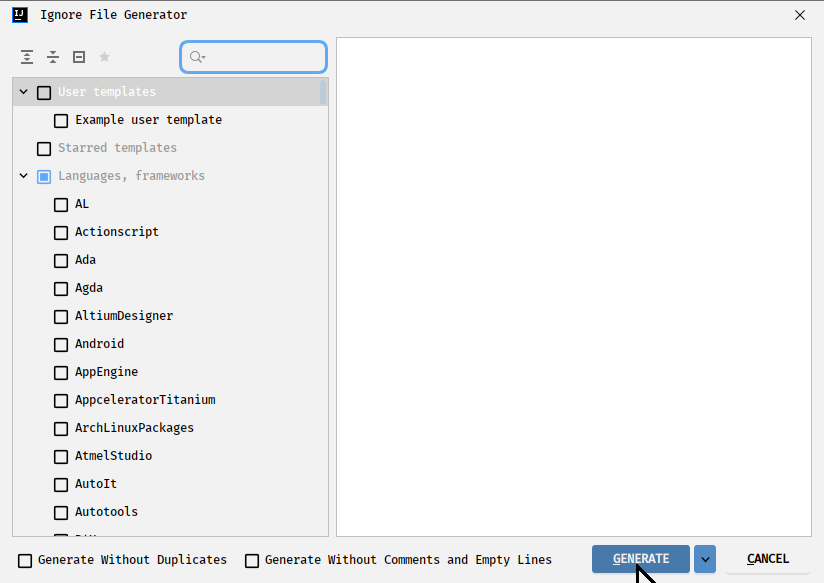
\includegraphics[width=0.7\textwidth]{img/oop/tdd/gradle/idea64_gitignore_generate.png}
    \caption{Generación del \texttt{.gitignore}}
    \label{fig:gitignore-generate}
  \end{figure}

  Con esto, podemos hacer \textit{commit} de los cambios que hicimos al proyecto.

  \begin{powershell}
    git add .
    git commit -m "PROJECT Adds Gradle configuration"
  \end{powershell}